\chapter{Sprint 4 - Design and implementation}

\section*{Introduction}
\addcontentsline{toc}{section}{Introduction}


In Sprint 4, we focused on the system management capabilities within the Odoo ERP system. This sprint aimed to provide administrators with the ability to manage the system, including app installation, user management, and setting access rights.

\section{Sprint 4 Backlog}
This sprint focuses on enhancing system management capabilities within the Odoo ERP. Table \ref{tab:sprint4_backlog} details the tasks planned for this sprint, outlining their respective durations.
\begin{longtable}{|c|p{8cm}|c|}
    \hline
    \rowcolor{purple!20} \textbf{N°} & \textbf{Tasks} & \textbf{Duration} \\ \hline
    \endfirsthead
    \hline
    \rowcolor{purple!20} \textbf{N°} & \textbf{Tasks} & \textbf{Duration} \\ \hline
    \endhead
    1 & As an administrator, I can install and manage apps. & 4 Day \\ \hline
    2 & As an administrator, I can create, update, and delete user accounts. & 4 Day \\ \hline
    3 & As an administrator, I can manage access rights and permissions for users. & 6 Days \\ \hline
    \caption{Sprint 4 Backlog for System Management}
    \label{tab:sprint4_backlog}
\end{longtable}

\section{Functional Specifications}

\subsection{Use Case Diagram}
This section presents the functional specifications for the System Management module.

Figure \ref{fig:sprint4_use_case_diagram} illustrates the Use Case Diagram specifically designed for Sprint 4.

\begin{figure}[h]
    \centering
    \makebox[\textwidth][c]{%
        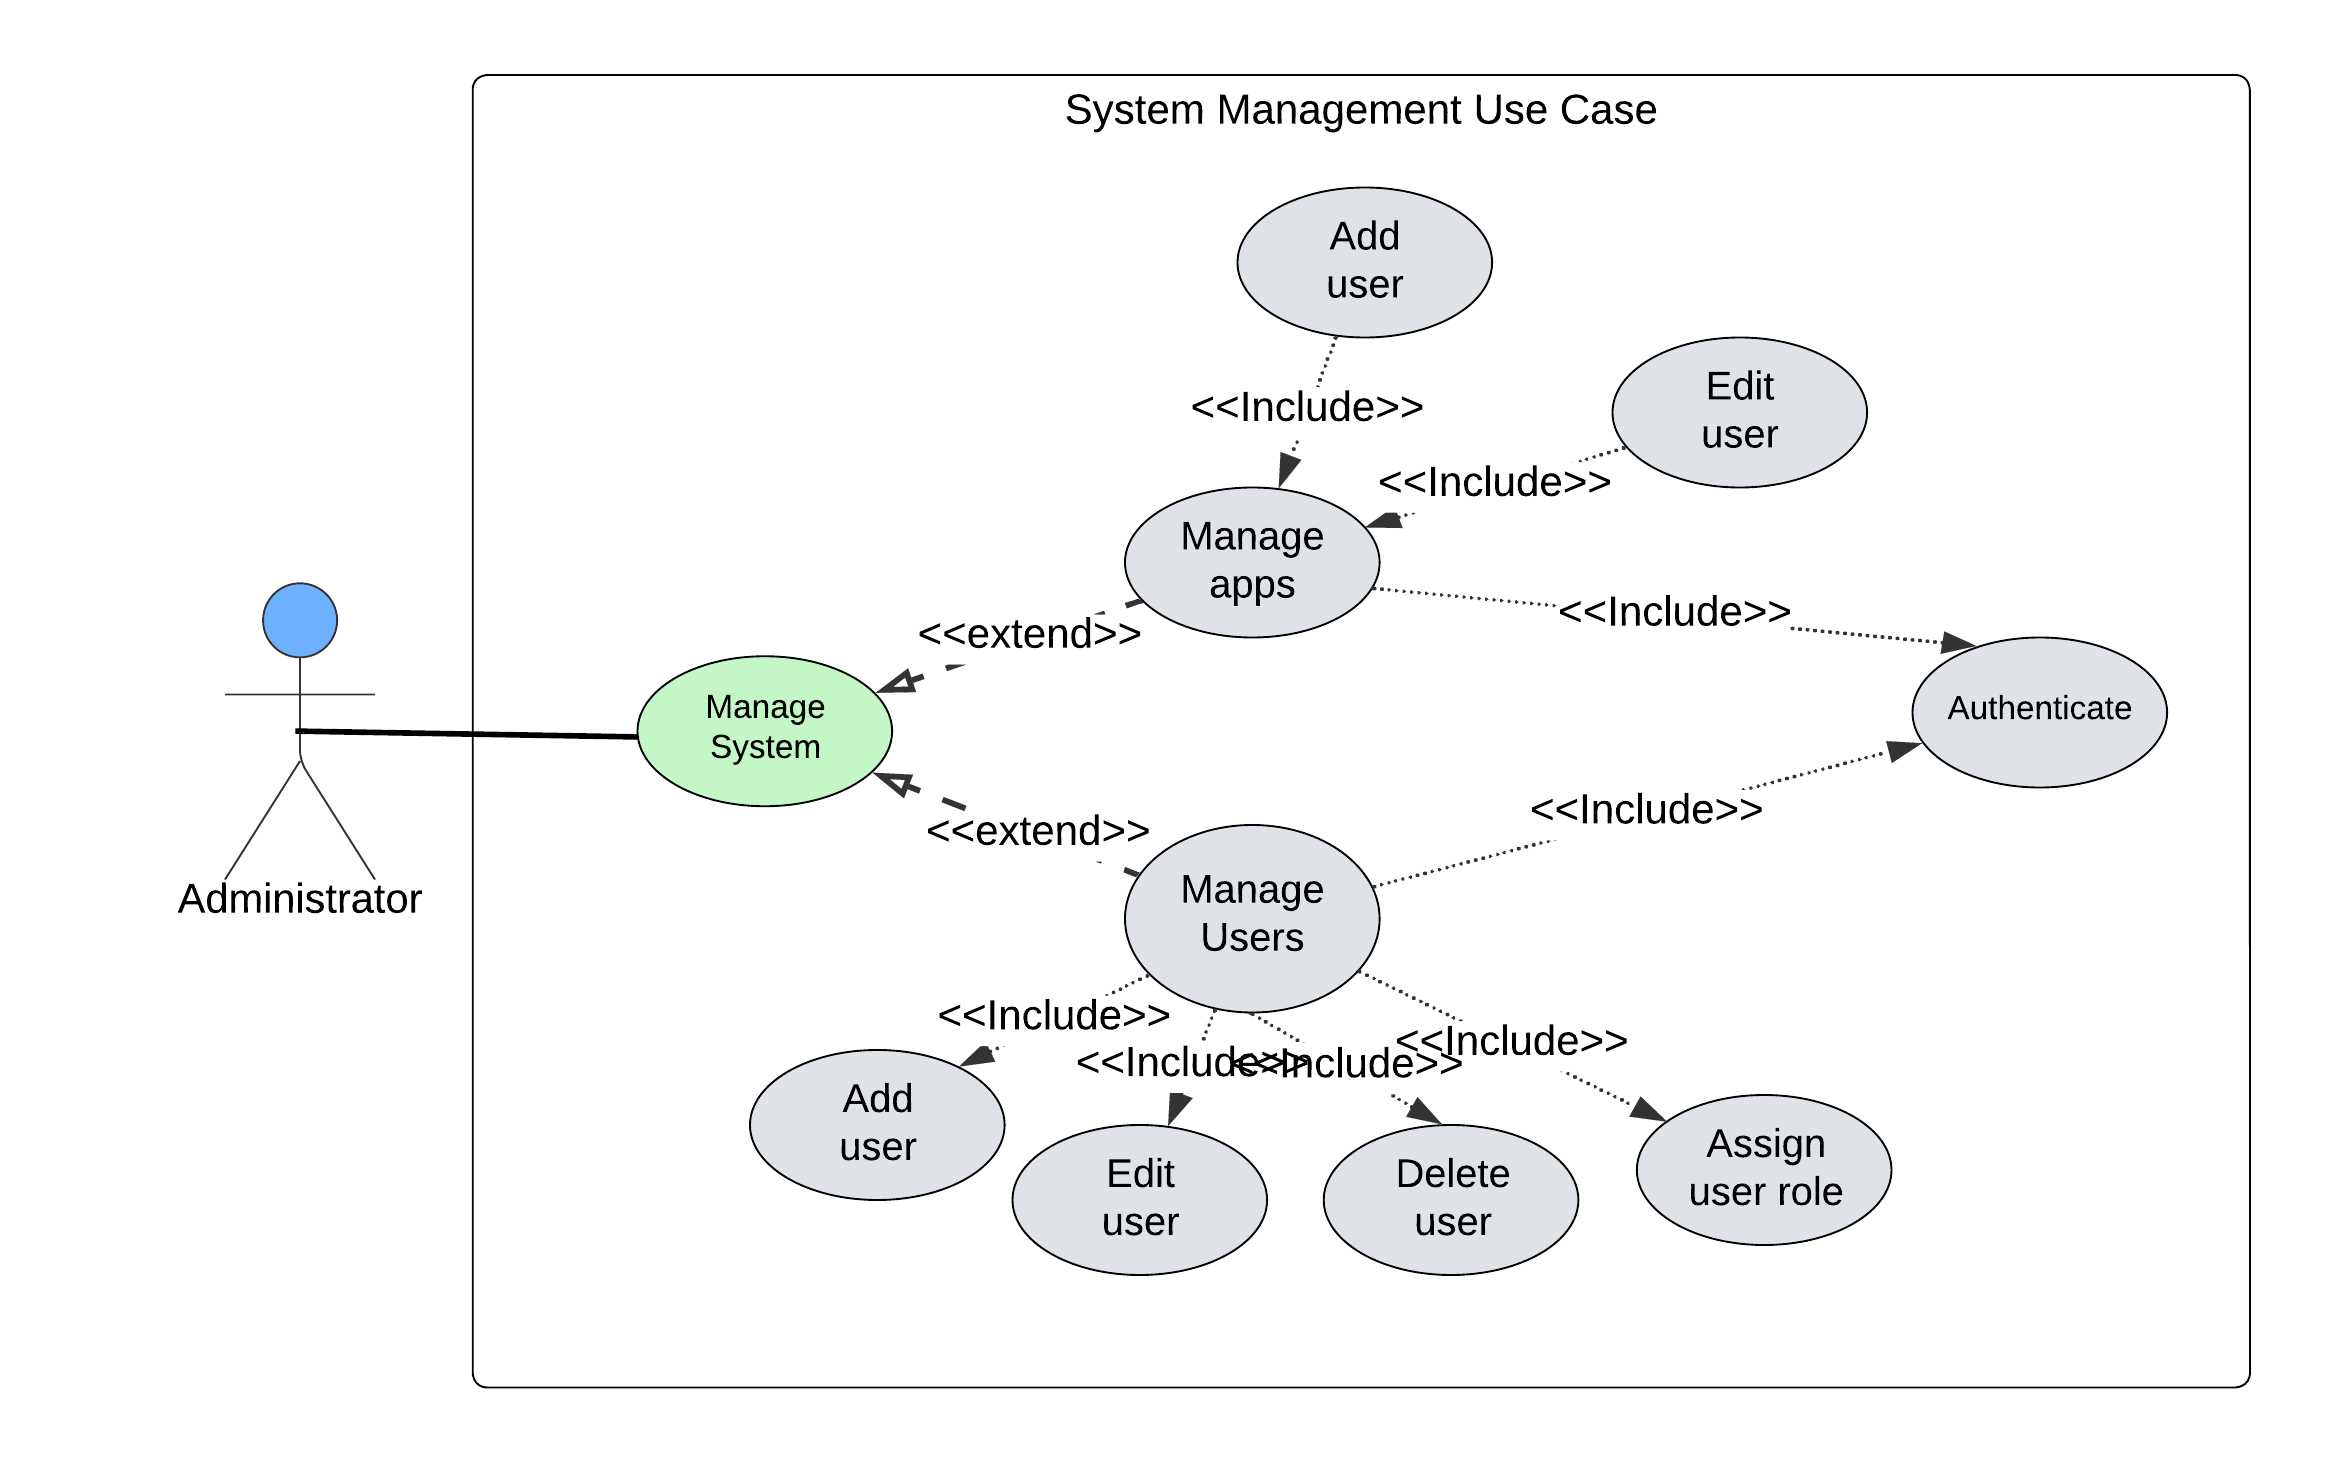
\includegraphics[width=1.2\textwidth]{sprint4/sprint4usecase.png}} % replace with your image path
    \caption{Sprint 4 Use Case Diagram}
    \label{fig:sprint4_use_case_diagram}
\end{figure}

\subsection{System Management Sequence Diagrams}
The sequence diagrams below illustrate the processes of installing an app and managing user accounts.

\begin{itemize}
    \item Administrator installs and manages apps.
    \item Administrator creates, updates, and deletes user accounts.
    \item Administrator sets access rights and permissions.
\end{itemize}

Figure \ref{fig:system_management_sequence_diagram} depicts the Sequence Diagram for managing system functionalities.

\begin{figure}[h]
    \centering
    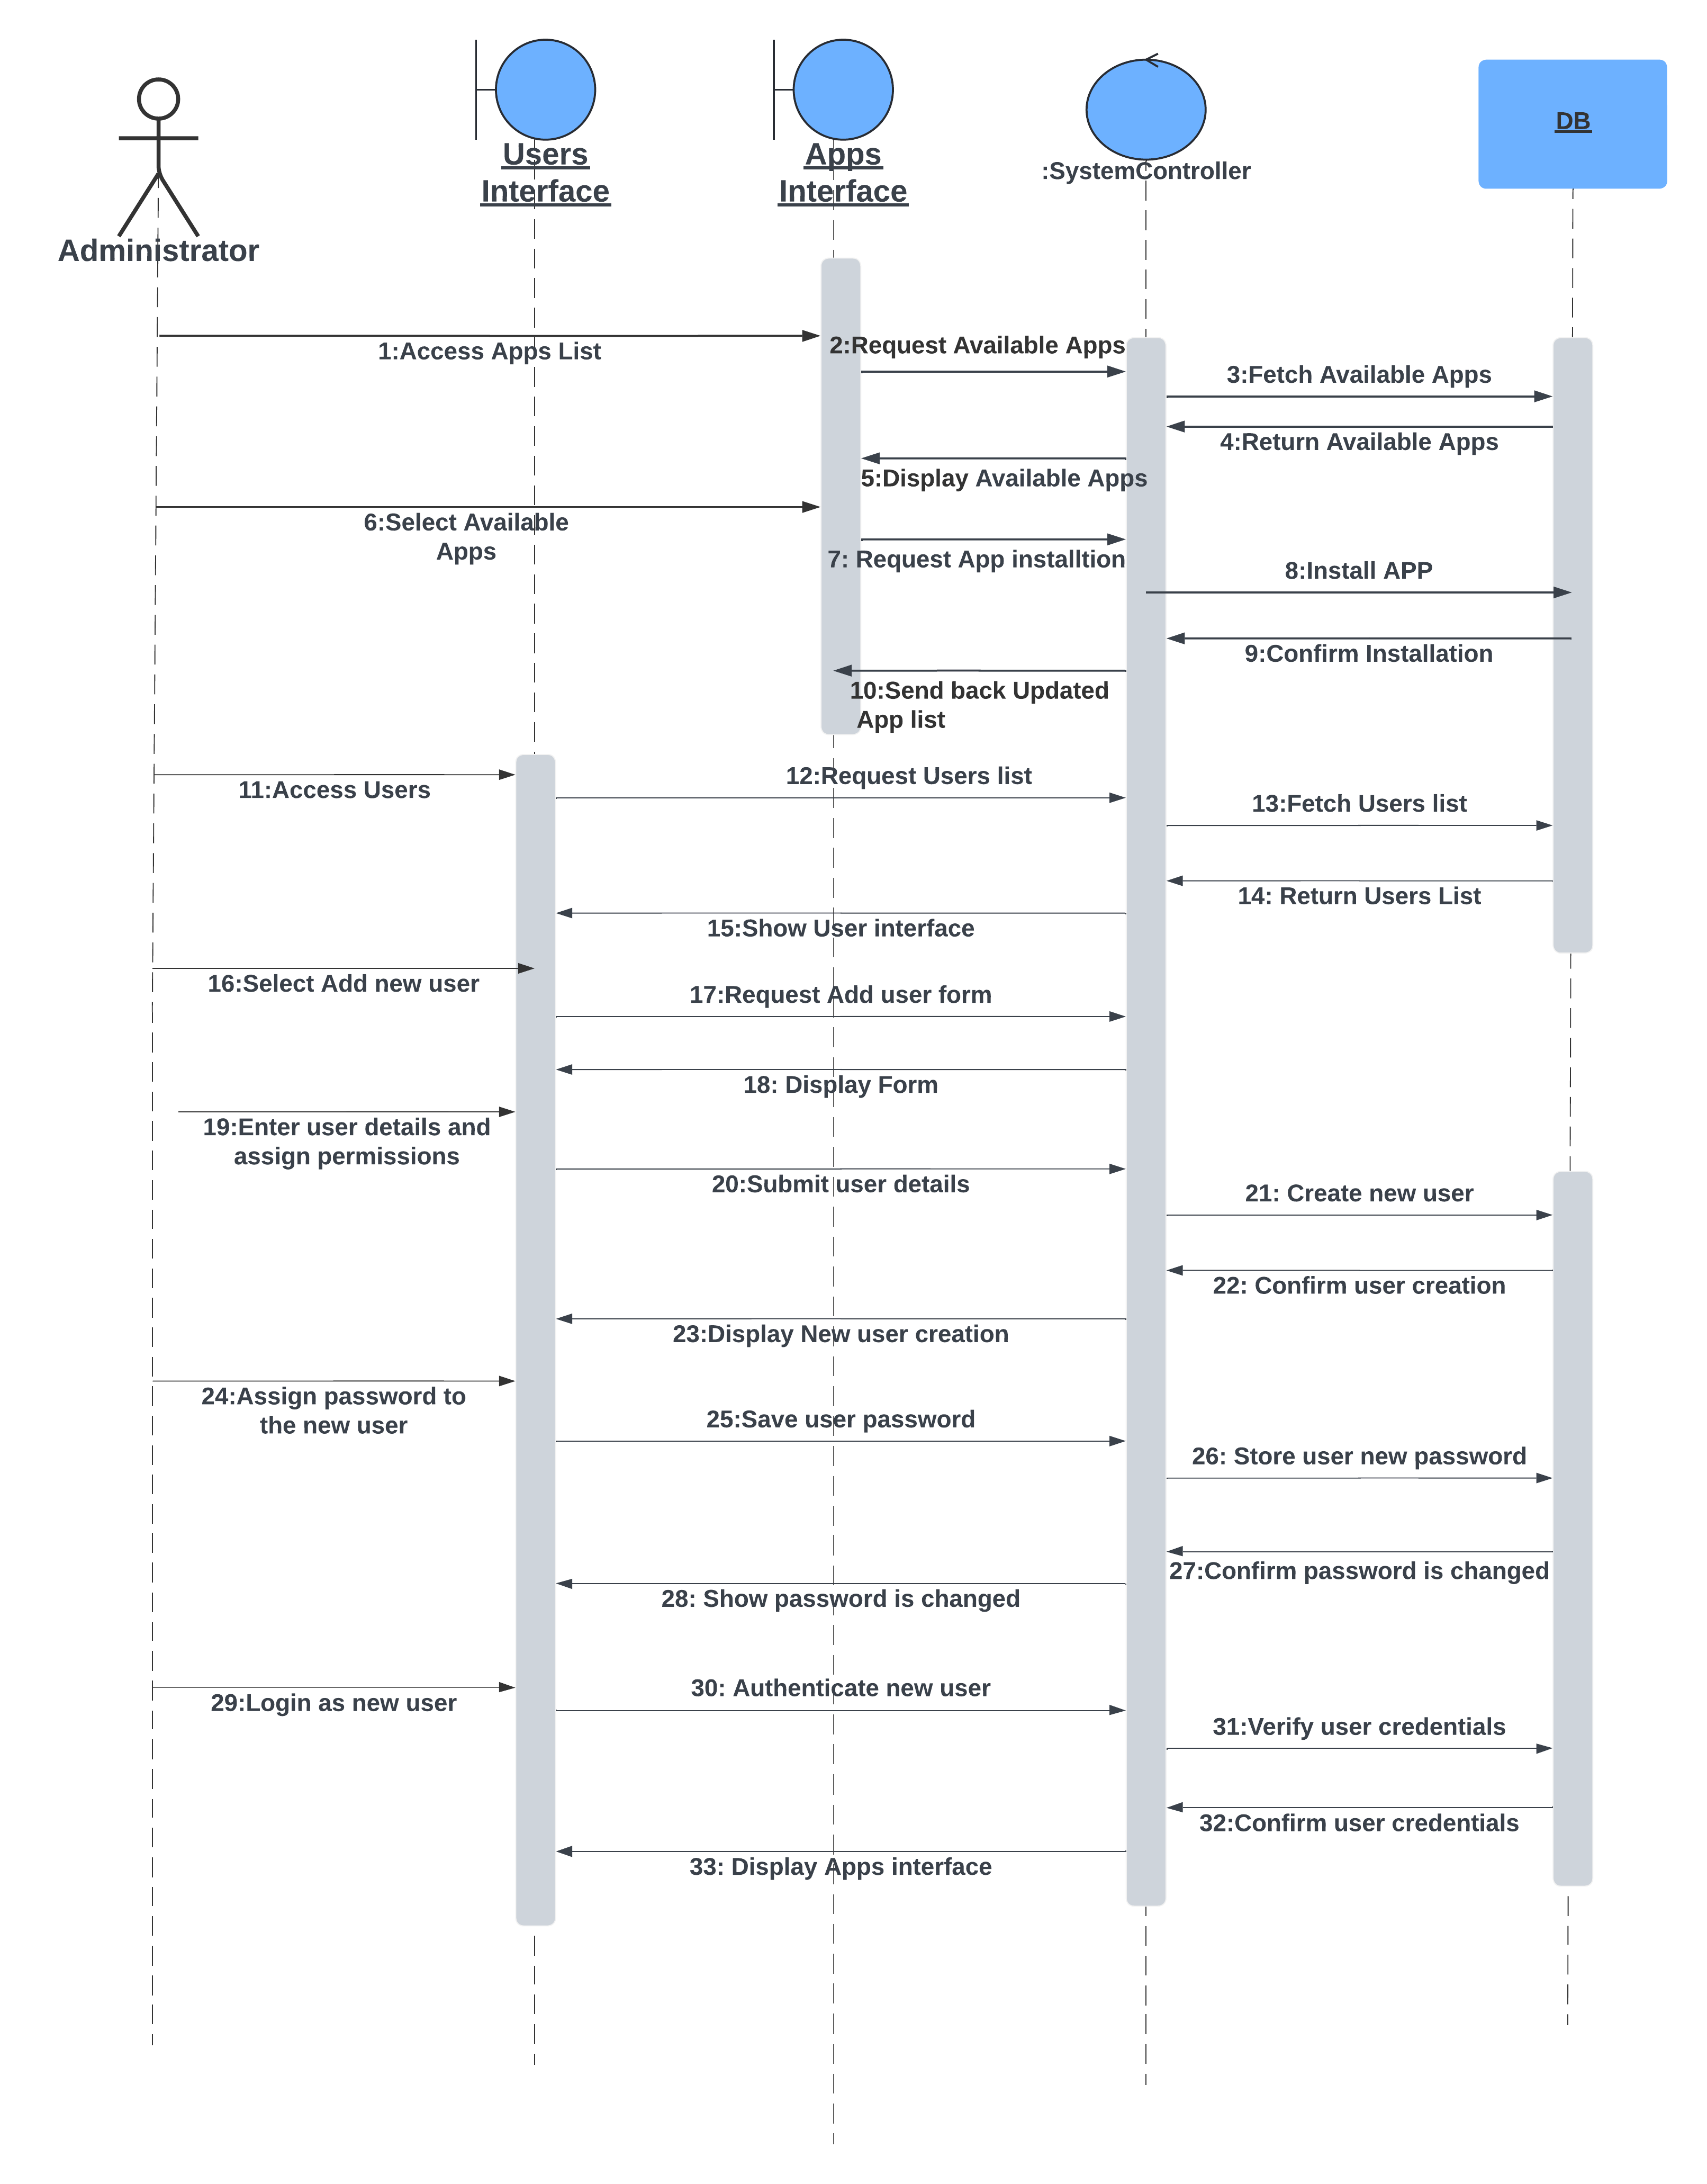
\includegraphics[width=0.7\textwidth]{sprint4/sprint4sequence.png} % replace with your image path
    \caption{Sequence Diagram for "System Management"}
    \label{fig:system_management_sequence_diagram}
\end{figure}
\section{Sprint Realization}

\subsection{System Management Screenshots}
\newpage
\subsection{App Interface}
Figure \ref{fig:app_interface} shows the system app interface where the administrator can upgrade or delete apps.

\begin{figure}[h]
    \centering
    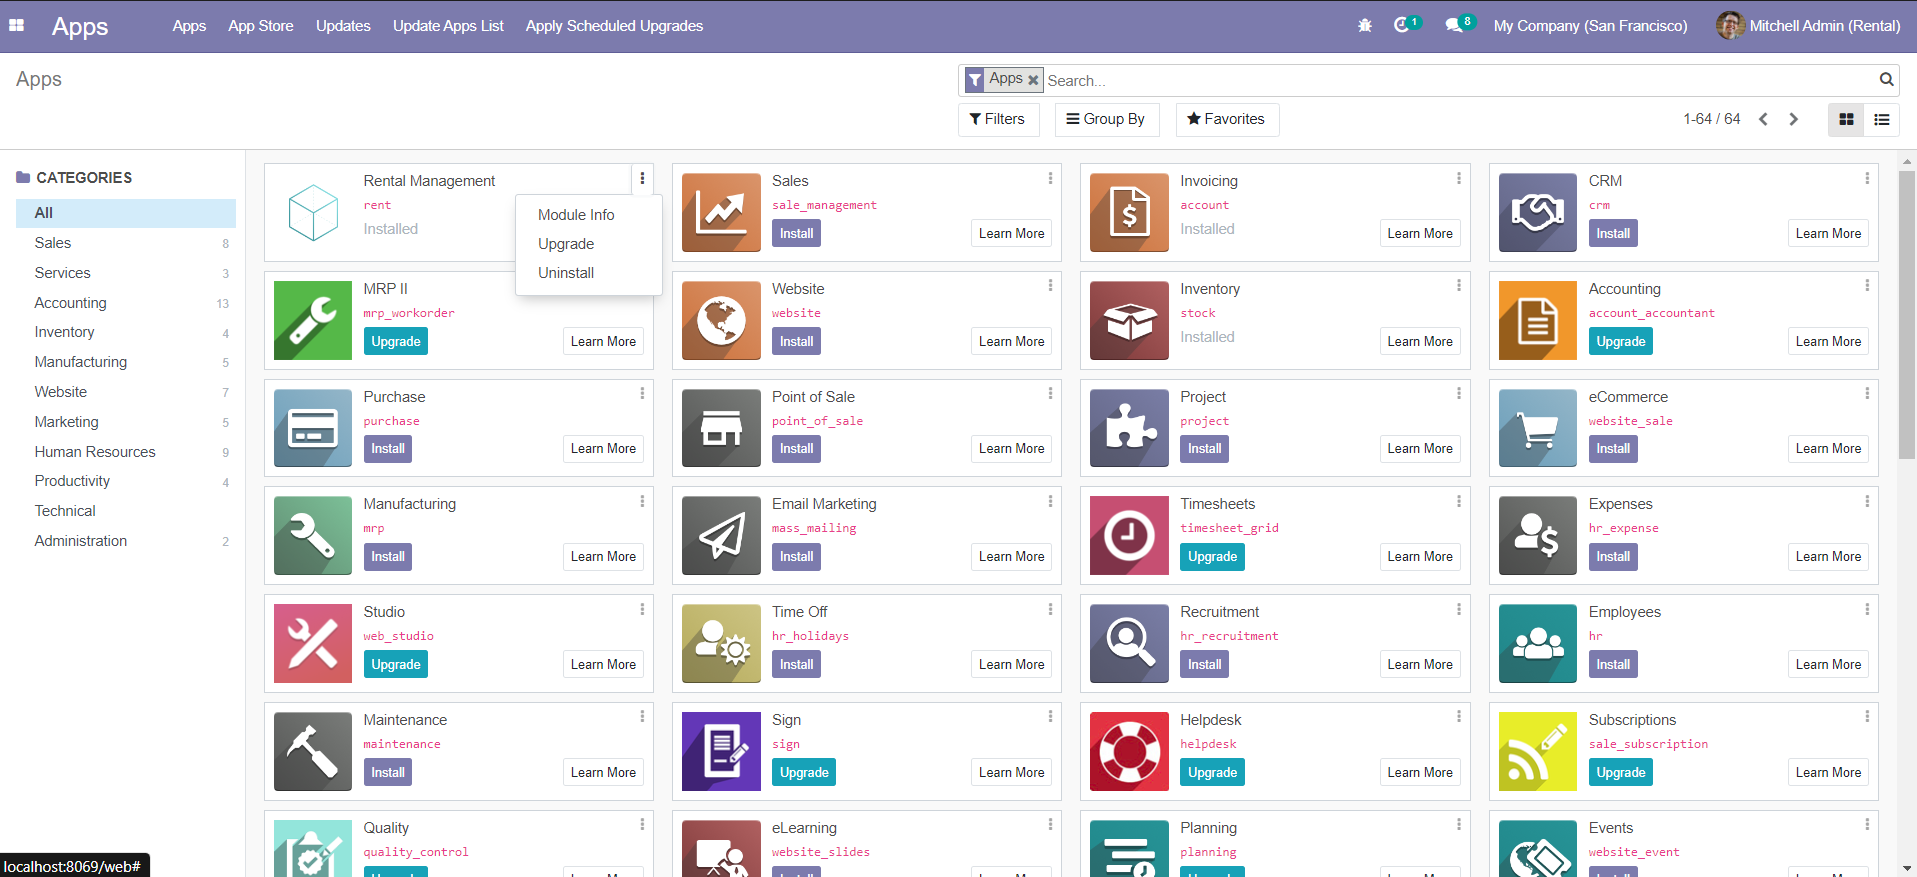
\includegraphics[width=1\textwidth]{sprint4/managesystem1.png} % replace with your image path
    \caption{Screenshot of the App Interface for Administrators}
    \label{fig:app_interface}
\end{figure}

\subsection{User Interface}
Figure \ref{fig:user_interface} presents the user interface showing the basic information of users.

\begin{figure}[h]
    \centering
    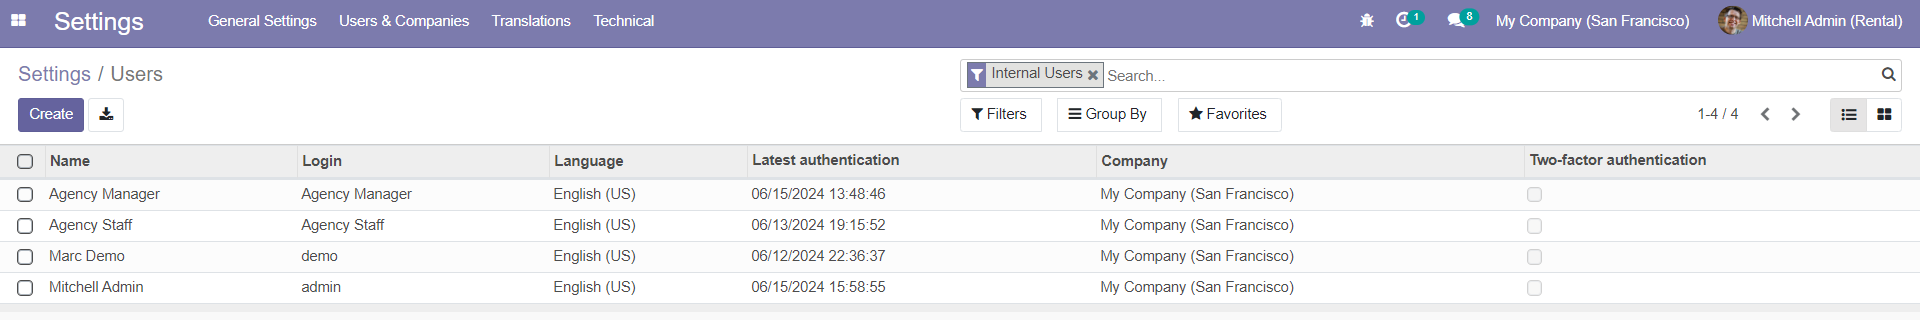
\includegraphics[width=1\textwidth]{sprint4/managesystem2.png} % replace with your image path
    \caption{Screenshot of the User Interface}
    \label{fig:user_interface}
\end{figure}
\newpage
\subsection{Adding a New User}
Figure \ref{fig:add_user_form} shows the form to add a new user, including assigning the right to manage the rental app.

\begin{figure}[h]
    \centering
    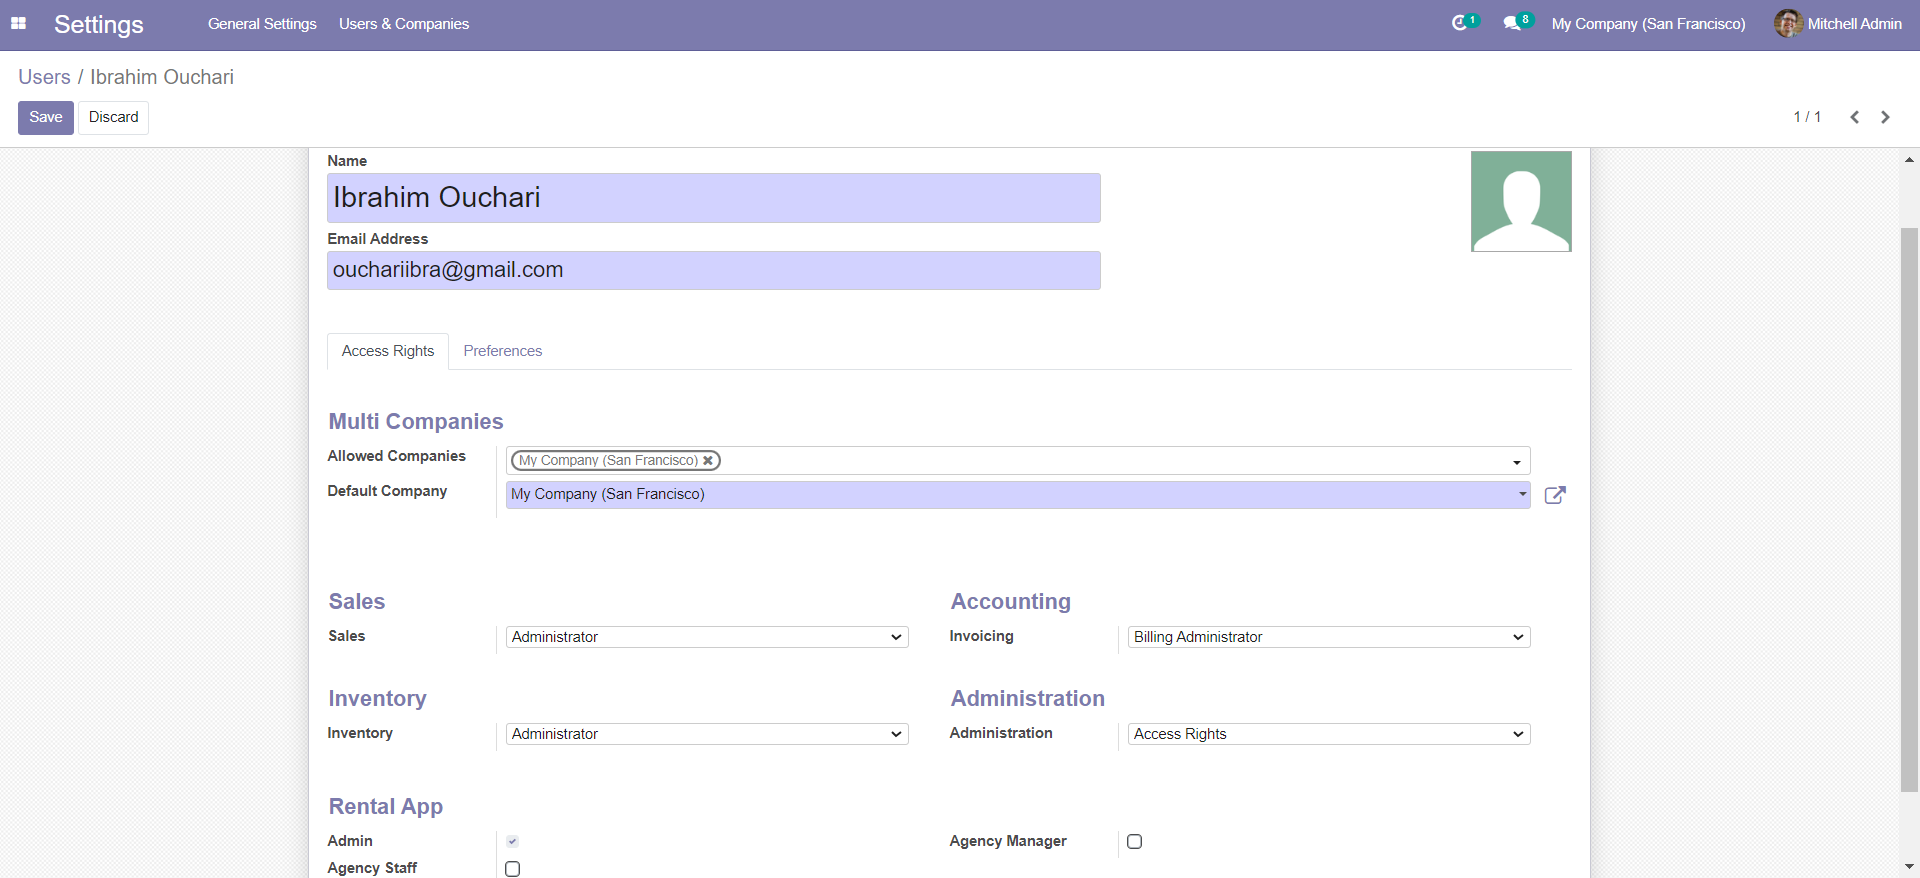
\includegraphics[width=1\textwidth]{sprint4/managesystem3.png} % replace with your image path
    \caption{Filling Out the Form to Add a New User}
    \label{fig:add_user_form}
\end{figure}

\subsection{Assigning a Password}
Figure \ref{fig:assign_password} illustrates the process of assigning a password to the newly created user.

\begin{figure}[h]
    \centering
    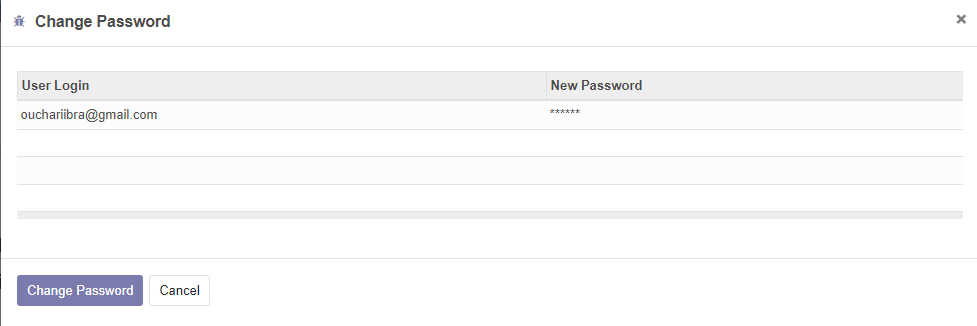
\includegraphics[width=1\textwidth]{sprint4/managesystem4.png} % replace with your image path
    \caption{Assigning a Password to the New User}
    \label{fig:assign_password}
\end{figure}
\newpage
\subsection{Logging In as the New User}
Figure \ref{fig:login_new_user} depicts logging into the app using the newly created account.

\begin{figure}[h]
    \centering
    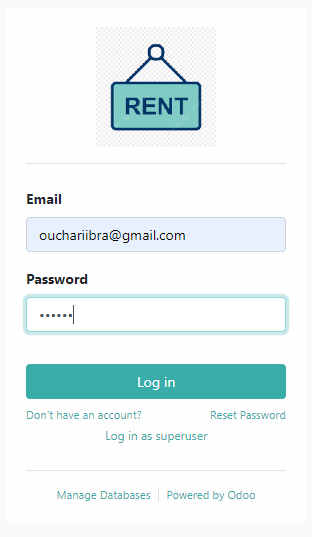
\includegraphics[width=0.2\textwidth]{sprint4/managesystem5.png} % replace with your image path
    \caption{Logging In with the Newly Created Account}
    \label{fig:login_new_user}
\end{figure}

\subsection{User Interface for New Account}
Figure \ref{fig:new_account_interface} shows the interface while using the newly created account.

% \begin{figure}[h]
%     \centering
%     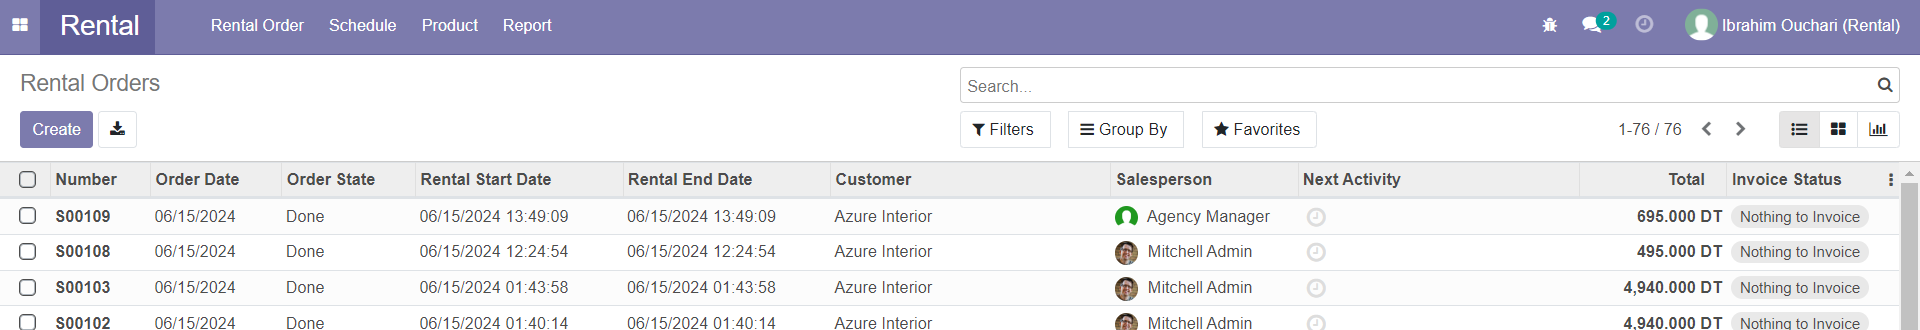
\includegraphics[width=1\textwidth]{sprint4/managesystem6.png} % replace with your image path
%     \caption{User Interface with the Newly Created Account}
%     \label{fig:new_account_interface}
% \end{figure}
\begin{figure}[h]
    \centering
    \makebox[\textwidth][c]{%
        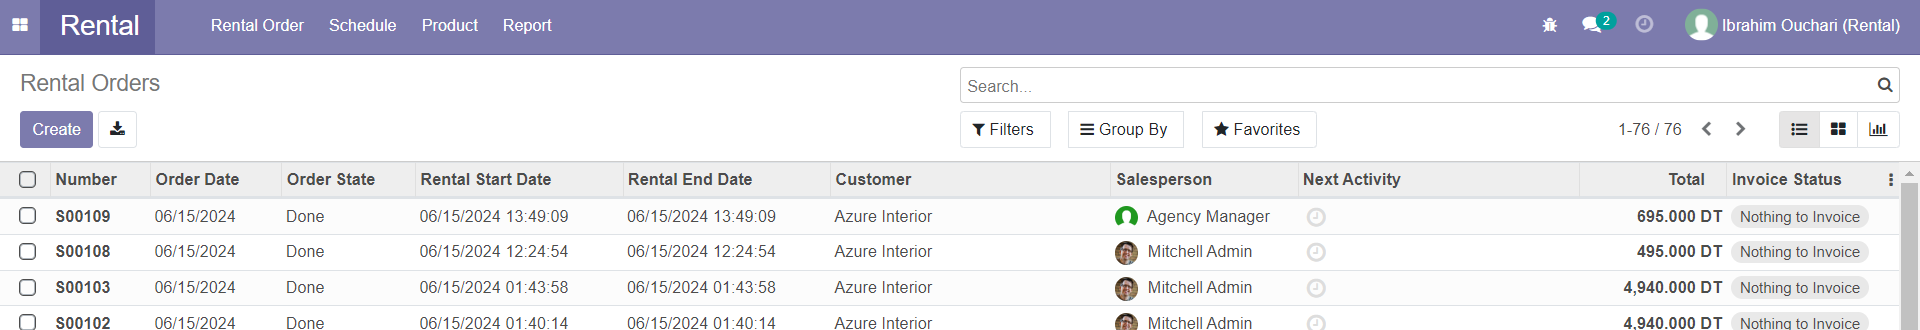
\includegraphics[width=1.2\textwidth]{sprint4/managesystem6.png}} % replace with your image path
    \caption{User Interface with the Newly Created Account}
    \label{fig:new_account_interface}
\end{figure}
\newpage
\section*{Conclusion}
\addcontentsline{toc}{section}{Conclusion}

In Sprint 4, we focused on enhancing the system management capabilities in Odoo ERP, allowing administrators to install and manage apps, create and manage user accounts, and set access rights and permissions. These functionalities enable efficient system management. The next sprint will continue to refine these capabilities and ensure smooth integration with other modules.
